\documentclass[UTF8]{ctexart}
\usepackage{amsmath, amsthm, amssymb, graphicx, amsfonts, indentfirst, subfigure}
\usepackage{fancyhdr,color,framed,enumitem}
\usepackage[perpage]{footmisc}
\usepackage{multirow}
\usepackage[table,xcdraw]{xcolor}
\linespread{1.5}
\usepackage[letterpaper,top=2cm,bottom=2cm,left=3cm,right=3cm,marginparwidth=1.75cm]{geometry}
\usepackage[colorlinks,
            linkcolor=blue,
            anchorcolor=blue,
            citecolor=blue]{hyperref}
\usepackage{hhline}
\usepackage{xcolor}
\usepackage{colortbl}
%It sets your colour line and then sets back to default (black)
%\ctexset{subsubsection = {number=\arabic{subsubsection}}}       %subsubsection形式改为1，2，3，...
\title{\Huge{北京大学自行车协会\protect\\25冬训手册}}
\date{\today}
\author{文体部}
\setlength{\parindent}{4pt}
\setlength{\headheight}{27pt}
\pagestyle{fancy}
\begin{document}
\maketitle

\begin{figure}[h]
    \centering
    \includegraphics*{会徽.png}
\end{figure}


\clearpage
\tableofcontents
\clearpage

\section{冬训目标}

冬训致力于提高会员体能，严明团队纪律，促进会员交流，培养团队责任感，从而锻炼出能胜任500 公里冬游的团队，为日后2000公里的暑期远征打下坚实的基础。

\section{冬训内容}

冬训包括为期8周的五四训练、海淀公园绕圈训练、四次单日拉练和四次相应的前站、骑行讲座、历史讲座、冬训体测、圣诞晚会暨冬训总结大会以及其他相关活动。

冬训一前将举办三日拉练，慕田峪拉练及前站，社考拉练，但\textbf{不计入冬训考勤}


\subsection{五四训练}

周一、三、五的五四训练于晚20:30在本部五四体育场跑道西侧会旗下集合签到，20:45签到结束并开始训练。按规定完成训练内容后训练记录一次五四训练考勤。

医学部同学因有晚课无法在集合时间前到达五四操场，需提前与【温瑶】（大水群搜索【温瑶】）联系说明情况并在21：00前到达，向队长说明后即可入队。

如遇恶劣天气等特殊情况，文体部会于训练当日20:00前在论坛工作区和大水群通知，改变训练场地或者取消训练。如果训练取消，将于11月25日安排补训，如取消的次数大于一次，只补训一次，多于一次的部分为所有会员计入考勤。

特殊情况的考勤记录和五四训练的纪律要求请见\href{https://chexie.net/bbs/content/index.php?bid=1\&tid=9576\&p=1}{\textit{【文体部】五四训练纪律要求}}。

\subsubsection{考勤作弊}
五四训练考勤作弊是指会员在未全程参与训练的情况下，获得当次训练考勤的行为。如果任何会员由于时间、身体等原因未能完成全部训练，应当向当次队长或文体部说明情况，当次考勤酌情减为半次或不计。如果出现(包括但不限于)以下情况，一律定义为考勤作弊:


\textit{1、在训练迟到的情况下不告知队长并直接补签;}

\textit{2、未完成一次训练中队长要求的所有项目，获得了当次训练签到，且没有在训练结束后一天之内告知当次训练队长或文体部。}

考勤作弊处罚详见\href{https://chexie.net/bbs/content/index.php?bid=1\&tid=9576\&p=1}{\textit{【文体部】五四训练纪律要求}}

冬训具有严肃性，需要保持高度的纪律，所有参加冬训的会员都需要遵守冬训的纪律。在此，望每位参加冬训的会员仔细阅读\href{https://chexie.net/bbs/content/index.php?bid=1\&tid=9576\&p=1}{\textit{【文体部】五四训练纪律要求}}。


\subsection{海淀公园绕圈训练}

周二或周四的海淀公园绕圈训练将在训练前2天13:00开放报名，在训练前1天13:00截止。每次训练会有人数限制，报名截止后领队将根据报名顺序拉群，入选后视为报名成功。按规定完成训练内容后记录一次海淀公园绕圈训练考勤。

如遇恶劣天气等特殊情况，文体部会于训练当日20:00前在当次训练群中通知取消训练，\textbf{不计考勤}。取消的训练\textbf{不予补训}，请需要冬训考勤的会员注意。

海淀公园绕圈训练的纪律要求请见\href{https://www.chexie.net/bbs/content/?bid=1&tid=9743&p=1}{\textit{【文体部】海淀公园绕圈训练通知}}。

\subsection{拉练}

每周末将开展单日拉练，每次拉练均有对应的前站。每次单日拉练或前站记录一次拉练考勤。

如遇恶劣天气等特殊情况，当次拉练队长将根据实际情况修改拉练终点、推迟或取消拉练。如果拉练取消，为所有成功报名（不含在队长通知前已经退出的）当次拉练的会员计入考勤。

拉练的纪律要求和处罚条例请见当次拉练通知帖、\href{https://chexie.net/bbs/content/?bid=1&tid=9618&p=1}{\textit{北京大学自行车协会出行条例（2023年10月修订）}}和\href{https://chexie.net/bbs/content/?bid=1&tid=9260&p=1}{\textit{北京大学自行车协会纪律处罚条例（2022年10月修订）}}。

\subsection{讲座}


冬训期间将开展一次骑行讲座和一次历史讲座。

骑行讲座为针对骑行知识所进行的讲座，需要参加往年或本年度的任意一次方可记录\textbf{本次冬训骑行讲座考勤}。

历史讲座为对协会历史的介绍讲座，必须要参加\textbf{本年度冬训历史讲座}方可记录\textbf{本次冬训历史讲座考勤}。

如因时间冲突等导致未能参加讲座的，请在讲座后联系讲座主讲人，按主讲人要求完成\textbf{补考勤任务}，完成后视为考勤成功。

讲座地点以及具体时间会在讲座前于论坛工作区公布。

\subsection{体测}

冬训体测为跑步体测，其中女生耐力跑3km，男生耐力跑4km。每人只有2次测试机会，一旦起跑视为使用了1次机会。指定测试时间段外会安排一次补测，补测时间会和体测其他具体安排在体测前于论坛工作区公布。

如果规定时间内无法参加，可以联系\textbf{冬训体测负责}（见论坛工作区），根据实际情况安排时间补测。

跑步体测积分标准如下：

\begin{table}[h]
    \centering
    \begin{tabular}{|c|c|c|}
    \hline
    女生3km用时X以内 & 男生4km用时X以内 & 积分 \\ \hline
    16min30s   & 19min      & 18 \\ \hline
    16min45s   & 19min15s   & 17 \\ \hline
    17min      & 19min30s   & 16 \\ \hline
    17min15s   & 19min45s   & 15 \\ \hline
    17min30s   & 20min      & 14 \\ \hline
    17min45s   & 20min15s   & 13 \\ \hline
    18min      & 20min30s   & 12 \\ \hline
    18min15s   & 20min45s   & 11 \\ \hline
    18min30s   & 21min      & 10 \\ \hline
    18min45s   & 21min15s   & 9  \\ \hline
    19min      & 21min30s   & 8  \\ \hline
    19min15s   & 21min45s   & 7  \\ \hline
    19min30s   & 22min      & 6  \\ \hline
    \end{tabular}\label{test}
    \end{table}

\textit{只要参加足够的训练，冬训几乎不会因为体测无法通过。} 

\section{通过冬训的标准}

冬训采用累计积分制，通过获得训练和拉练考勤积分，部分考勤可以互抵。通过冬训需要满足积分要求，参加完整体测，获得骑行讲座和历史讲座考勤。细则如下。


\subsection{冬训积分标准}
冬训采用累计积分制，积分标准如下：

\begin{itemize}[nosep,left=4em]
    \item \textbf{五四训练积分} \ 每次五四训练考勤积1分；
    \item \textbf{海淀公园绕圈训练积分} \ 每次海淀公园绕圈训练考勤积1分；
    \item \textbf{拉练积分} \  每次单日拉练积2分，每次前站拉练积2分；
    \item \textbf{体测积分} \  体测积分标准请见\ref{test}。 
\end{itemize}

\subsection{冬训通过标准}

满足以下\textbf{所有}条件即视为通过25冬训：
\begin{enumerate}[nosep,left=4em]
    \item 训练积分（$=\text{五四训练积分}+\text{海淀公园绕圈训练积分}$）$\ge 8$分，其中五四训练积分$\ge 6$分，后9次五四训练积分$\ge 3$分\footnote{也即至少参加6次五四训练，其中后7次五四训练至少参加3次。}；
    \item 拉练积分$\ge 4$分；
    \item 参加冬训体测或补测，且至少完成一次完整的体测\footnote{即女生完整完成3km，男生完整完成4km。}；
    \item 总积分（$=\text{训练积分}+\text{拉练积分}+\text{体测积分}$）$\ge 30$分；
    \item 获得本次冬训骑行讲座、历史讲座考勤。
\end{enumerate}

\subsection{考勤互抵}

部分考勤可以互抵，考勤互抵标准如下：

\begin{itemize}[nosep,left=4em]
    \item 1次前站考勤可抵1次五四训练考勤（此时该次前站不再计入拉练考勤和积分）；
    \item 最多使用前站考勤抵1次后9次五四训练考勤。 
\end{itemize}

\subsection{举例}
\small{
    \textbf{例1} \ 现有会员A，男生，参加了2次海淀公园绕圈训练，6次五四训练，其中后9参加了2次；去了1次前站和3次正式拉练；跑步体测19min20s；参与了去年春天的骑行讲座和本次冬训的历史讲座。

如果A不进行考勤互抵，将由于后9次五四训练积分只有2分而无法通过冬训。
如果A进行考勤互抵，使用1次前站考勤抵1次后7次五四训练考勤，那么
\begin{enumerate}[nosep,left=4em]
    \item 训练积分（$=\text{五四训练积分}+\text{海淀公园绕圈训练积分}=7+2$）$=9\ge 8$分，其中五四训练积分$=7\ge 6$分，后7次五四训练积分=3$\ge 3$分；
    \item 拉练积分$=6\ge 4$分；
    \item 参加冬训体测或补测，且至少完成一次完整的体测；
    \item 总积分（$=\text{训练积分}+\text{拉练积分}+\text{体测积分}$）$=9+6+16=31\ge 30$分；
    \item 获得本次冬训骑行讲座、历史讲座考勤。
\end{enumerate}

会员A通过冬训。\\
}

\small{
    \textbf{例2} \ 现有会员B，女生，参加了4次海淀公园绕圈训练，16次五四训练，其中后9次参加了7次；去了1次前站和4次正式拉练；跑步体测19min48s；参与了本次冬训的骑行讲座和历史讲座。

那么
\begin{enumerate}[nosep,left=4em]
    \item 训练积分（$=\text{五四训练积分}+\text{海淀公园绕圈训练积分}=16+4$）$=20\ge 8$分，其中五四训练积分$=16\ge 6$分，后7次五四训练积分=7$\ge 3$分；
    \item 拉练积分$=10\ge 4$分；
    \item 参加冬训体测或补测，且至少完成一次完整的体测；
    \item 总积分（$=\text{训练积分}+\text{拉练积分}+\text{体测积分}$）$=20+10+0=30\ge 30$分；
    \item 获得本次冬训骑行讲座、历史讲座考勤。
\end{enumerate}

会员B通过冬训。

}



\section{其他需要说明的事项}

\subsection{关于冬游}

冬游是每年寒假协会组织的官方的骑行活动，一般为期6至10天，组队长途骑行。获得冬游资格的会员才可以参加冬游。

获得冬游资格有以下三种方式：
\begin{enumerate}[nosep,left=2em]
    \item 通过任意一次冬训或者春训；
    \item 参加过暑期远征的暑期队员；
    \item 如果出现重大伤病或变故导致无法通过当次冬训的会员，可以申请特批，特批通过后即可获得冬游资格\footnote{但不视作通过当次冬训。}。
\end{enumerate}

\subsection{关于冬训和暑期的关系}

冬训主要影响冬游，和暑期没有直接关系。如果通过冬训，可以减少春训的考勤次数。有关暑期队员选拔请见\href{https://chexie.net/bbs/content/?bid=1&tid=9610&p=1}{\textit{北京大学自行车协会暑期队员选拔条例（2012年2月修订）}}。
\clearpage
\appendix

\section{冬训拉练目的地简介}

\subsection{大运河}

通州大运河森林公园，国家AAAA级景区，世界文化遗产中国大运河的一部分。通州大运河是京杭大运河的起始端，大运河森林公园位于北京通州新城北运河两侧，是协会少有的向东出发的拉练。公园里风景很好，且拉练全程无坡。

\begin{figure}[h]
    \centering
    \subfigure{
    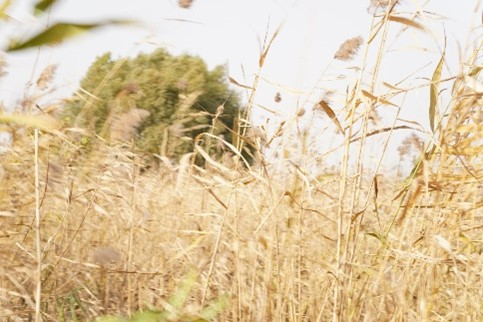
\includegraphics[width=0.45\textwidth]{大运河1.jpg} 
    }
    \quad
    \subfigure{
    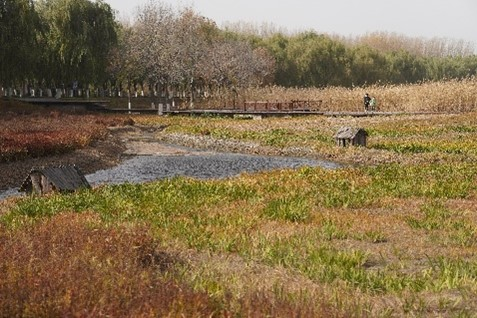
\includegraphics[width=0.45\textwidth]{大运河2.jpg} 
    }
    \end{figure}

\subsection{十三陵水库}

十三陵水库地处昌平区，为山区盆地水库，占地面积 751 公顷，其中陆地面积 440 公顷，水面 311 公顷。水库四周群山矗立，特别是北岸巍峨的蟒山拔地而起，宽 阔的水面，倒映群山，给人以“高峡出平湖”之感。山脚与水面的衔接处形成多处水 湾港汊，景色幽静宜人。

\begin{figure}[h]
    \centering
    \subfigure{
    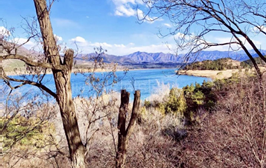
\includegraphics[width=0.45\textwidth]{十三陵水库1.png} 
    }
    \quad
    \subfigure{
    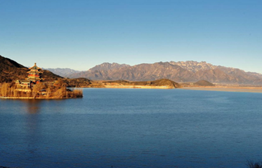
\includegraphics[width=0.45\textwidth]{十三陵水库2.png} 
    }
    \quad
    \end{figure}


\subsection{石花洞}

北京石花洞国家地质公园位于北京市房山区河北镇南车营村，距京城55公里。

石花洞原名“潜真洞”，自发现至今已500多年。因洞内雕有三尊大理石佛像，曾改称“石佛洞”，香火曾盛极一时。石花洞是国内发现的岩溶洞穴中集规模大、洞层多、沉积类型全、次生化学沉积物数量大的洞穴，其美学价值和科研价值也可居世界洞穴前列。

\begin{figure}[h]
    \centering
    \subfigure{
    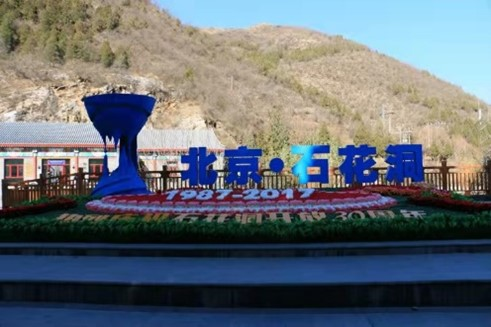
\includegraphics[width=0.45\textwidth]{石花洞1.jpg} 
    }
    \quad
    \subfigure{
    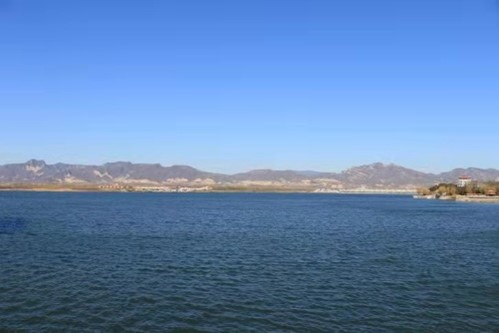
\includegraphics[width=0.45\textwidth]{石花洞2.jpg} 
    }
    \quad
    \end{figure}


\subsection{潭柘寺}

潭柘寺，位于北京西部门头沟区东南部的潭柘山麓，距市中心30 余公里。寺院坐北朝南，背倚宝珠峰，周围有九座高大的山峰呈马蹄环护，宛如在条巨龙的拥立之下。高大的山峰挡住了从西北方袭来的寒流，因此这里气候温暖、湿润，寺内古树参天，佛塔林立，殿宇巍峨，整座寺院建筑依地势而巧妙布局，错落有致，更有翠竹名花点缀。环境极为优美。

\begin{figure}[h]
    \centering
    \subfigure{
    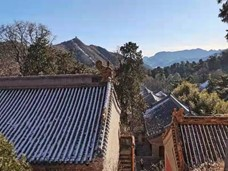
\includegraphics[width=0.45\textwidth]{潭柘寺1.jpg} 
    }
    \quad
    \subfigure{
    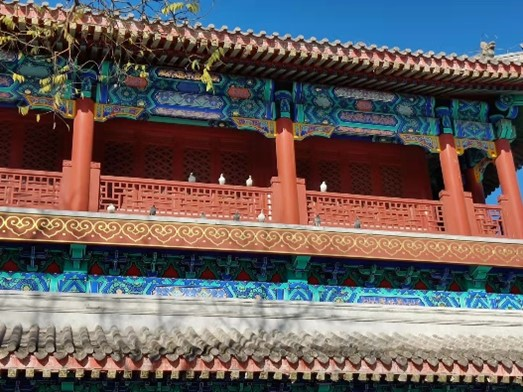
\includegraphics[width=0.45\textwidth]{潭柘寺2.jpg} 
    }
    \quad
    \end{figure}


\end{document}

